\chapter{Ergebnisse der Untersuchungen}




\begin{table}[h!]
\centering
\caption{Vergleich zwischen dem Betrieb mit 3MAF und HATCOL 4467.}
\label{tab:VergleichKMOele}
\begin{tabular}{|cC{3cm}C{3cm}|}
\hline

                                                                & 3MAF                        & HATCOL 4467 \\ \hline
\multicolumn{1}{|c|}{el. Leistung Verdichter {[}W{]}}           & \multicolumn{1}{c|}{2436}   & 2542        \\
\multicolumn{1}{|c|}{Leistung Verdampfer {[}W{]}}               & \multicolumn{1}{c|}{5383}   & 5442        \\
\multicolumn{1}{|c|}{Leistung Kondensator {[}W{]}}             & \multicolumn{1}{c|}{7589}   & 7882        \\
\multicolumn{1}{|c|}{EER}                                       & \multicolumn{1}{c|}{2.21}   & 2.14        \\ \hline
\multicolumn{1}{|c|}{Verdampfungstemperatur (K1) {[}°C{]}}      & \multicolumn{1}{c|}{-9.46}  & -9.96       \\
\multicolumn{1}{|c|}{Kondensationstemperatur (K1) {[}°C{]}}    & \multicolumn{1}{c|}{31.82}  & 34.51       \\
\multicolumn{1}{|c|}{Überhitzung (K1) {[}K{]}}                  & \multicolumn{1}{c|}{8.21}   & 7.77        \\
\multicolumn{1}{|c|}{Unterkühlung (K1) {[}K{]}}                 & \multicolumn{1}{c|}{0}      & 0           \\
\multicolumn{1}{|c|}{Dampfanteil vor EV (K1) {[}\%{]}}          & \multicolumn{1}{c|}{26}     & 20          \\
\multicolumn{1}{|c|}{Massenstrom (K1) {[}g/s{]}}                & \multicolumn{1}{c|}{8.34}   & 8.18        \\
\multicolumn{1}{|c|}{Druckabfall über Verdampfer (K1) {[}Pa{]}} & \multicolumn{1}{c|}{64531}  & 59450       \\ \hline
\multicolumn{1}{|c|}{Verdampfungstemperatur (K2) {[}°C{]}}      & \multicolumn{1}{c|}{-10.24} & -10.42      \\
\multicolumn{1}{|c|}{Kondensationstemperatur (K2) {[}°C{]}}    & \multicolumn{1}{c|}{33.82}  & 35.14       \\
\multicolumn{1}{|c|}{Überhitzung (K2) {[}K{]}}                  & \multicolumn{1}{c|}{8.19}   & 7.93        \\
\multicolumn{1}{|c|}{Unterkühlung (K2) {[}K{]}}                 & \multicolumn{1}{c|}{0}      & 0           \\
\multicolumn{1}{|c|}{Dampfanteil vor EV (K2) {[}\%{]}}          & \multicolumn{1}{c|}{16}     & 15          \\
\multicolumn{1}{|c|}{Massenstrom (K2) {[}g/s{]}}                & \multicolumn{1}{c|}{8.06}   & 8.03        \\
\multicolumn{1}{|c|}{Druckabfall über Verdampfer (K2) {[}Pa{]}} & \multicolumn{1}{c|}{63828}  & 62899       \\ \hline
\multicolumn{1}{|c|}{Verdampfungstemperatur (K3) {[}°C{]}}      & \multicolumn{1}{c|}{-10.25} & -10.54      \\
\multicolumn{1}{|c|}{Kondensationstemperatur (K3) {[}°C{]}}    & \multicolumn{1}{c|}{33.25}  & 34.67       \\
\multicolumn{1}{|c|}{Überhitzung (K3) {[}K{]}}                  & \multicolumn{1}{c|}{8.53}   & 8.90        \\
\multicolumn{1}{|c|}{Unterkühlung (K3) {[}K{]}}                 & \multicolumn{1}{c|}{0}      & 0           \\
\multicolumn{1}{|c|}{Dampfanteil vor EV (K3) {[}\%{]}}          & \multicolumn{1}{c|}{20}     & 16          \\
\multicolumn{1}{|c|}{Massenstrom (K3) {[}g/s{]}}                & \multicolumn{1}{c|}{8.05}   & 7.96        \\
\multicolumn{1}{|c|}{Druckabfall über Verdampfer (K3) {[}Pa{]}} & \multicolumn{1}{c|}{56099}  & 52894       \\ \hline
\multicolumn{1}{|c|}{Durchschnittsprodukttemperatur {[}°C{]}}   & \multicolumn{1}{c|}{5.35}   & 5.63        \\
\multicolumn{1}{|c|}{Maximale Produkttemperatur {[}°C{]}}       & \multicolumn{1}{c|}{10.54}  & 11.10       \\
\multicolumn{1}{|c|}{Minimale Produkttemperatur {[}°C{]}}       & \multicolumn{1}{c|}{0.98}   & 0.56        \\
\multicolumn{1}{|c|}{Einlasstemperatur Luft {[}°C{]}}           & \multicolumn{1}{c|}{7.68}   & 8.69        \\
\multicolumn{1}{|c|}{Auslasstemperatur Luft {[}°C{]}}           & \multicolumn{1}{c|}{-0.31}  & -0.02       \\ \hline
\end{tabular}
\end{table}




\clearpage



\begin{table}[h!]
\centering
\caption{Vergleich zwischen verschiedenen Abtauintervallen.}
\label{tab:Vergleich4h3h}
\begin{tabular}{|cC{3cm}C{3cm}|}
\hline
                                                                & 4h Abtauintervall           & Bedarfsabtauung \\ \hline
\multicolumn{1}{|c|}{el. Leistung Verdichter {[}W{]}}           & \multicolumn{1}{c|}{2542}   & 2554              \\
\multicolumn{1}{|c|}{Leistung Verdampfer {[}W{]}}               & \multicolumn{1}{c|}{5442}   & 5770              \\
\multicolumn{1}{|c|}{Leistung Kondensator {[}W{]}}             & \multicolumn{1}{c|}{7882}   & 8230              \\
\multicolumn{1}{|c|}{EER}                                       & \multicolumn{1}{c|}{2.14}   & 2.26              \\ \hline
\multicolumn{1}{|c|}{Verdampfungstemperatur (K1) {[}°C{]}}      & \multicolumn{1}{c|}{-9.96}  & -7.71             \\
\multicolumn{1}{|c|}{Kondensationstemperatur (K1) {[}°C{]}}    & \multicolumn{1}{c|}{34.51}  & 34.71             \\
\multicolumn{1}{|c|}{Überhitzung (K1) {[}K{]}}                  & \multicolumn{1}{c|}{7.77}   & 8.06              \\
\multicolumn{1}{|c|}{Unterkühlung (K1) {[}K{]}}                 & \multicolumn{1}{c|}{0}      & 0                 \\
\multicolumn{1}{|c|}{Dampfanteil vor EV (K1) {[}\%{]}}          & \multicolumn{1}{c|}{20}     & 23                \\
\multicolumn{1}{|c|}{Massenstrom (K1) {[}g/s{]}}                & \multicolumn{1}{c|}{8.18}   & 8.88              \\
\multicolumn{1}{|c|}{Druckabfall über Verdampfer (K1) {[}Pa{]}} & \multicolumn{1}{c|}{59450}  & 64649             \\ \hline
\multicolumn{1}{|c|}{Verdampfungstemperatur (K2) {[}°C{]}}      & \multicolumn{1}{c|}{-10.42} & -7.95             \\
\multicolumn{1}{|c|}{Kondensationstemperatur (K2) {[}°C{]}}    & \multicolumn{1}{c|}{35.14}  & 35.30             \\
\multicolumn{1}{|c|}{Überhitzung (K2) {[}K{]}}                  & \multicolumn{1}{c|}{7.93}   & 8.06              \\
\multicolumn{1}{|c|}{Unterkühlung (K2) {[}K{]}}                 & \multicolumn{1}{c|}{0}      & 0                 \\
\multicolumn{1}{|c|}{Dampfanteil vor EV (K2) {[}\%{]}}          & \multicolumn{1}{c|}{15}     & 20                \\
\multicolumn{1}{|c|}{Massenstrom (K2) {[}g/s{]}}                & \multicolumn{1}{c|}{8.03}   & 8.79              \\
\multicolumn{1}{|c|}{Druckabfall über Verdampfer (K2) {[}Pa{]}} & \multicolumn{1}{c|}{62899}  & 68890             \\ \hline
\multicolumn{1}{|c|}{Verdampfungstemperatur (K3) {[}°C{]}}      & \multicolumn{1}{c|}{-10.54} & -8.20             \\
\multicolumn{1}{|c|}{Kondensationstemperatur (K3) {[}°C{]}}    & \multicolumn{1}{c|}{34.67}  & 34.77             \\
\multicolumn{1}{|c|}{Überhitzung (K3) {[}K{]}}                  & \multicolumn{1}{c|}{8.90}   & 9.07              \\
\multicolumn{1}{|c|}{Unterkühlung (K3) {[}K{]}}                 & \multicolumn{1}{c|}{0}      & 0                 \\
\multicolumn{1}{|c|}{Dampfanteil vor EV (K3) {[}\%{]}}          & \multicolumn{1}{c|}{16}     & 21                \\
\multicolumn{1}{|c|}{Massenstrom (K3) {[}g/s{]}}                & \multicolumn{1}{c|}{7.96}   & 8.68              \\
\multicolumn{1}{|c|}{Druckabfall über Verdampfer (K3) {[}Pa{]}} & \multicolumn{1}{c|}{52894}  & 57693             \\ \hline
\multicolumn{1}{|c|}{Durchschnittsprodukttemperatur {[}°C{]}}   & \multicolumn{1}{c|}{5.63}   & 5.67              \\
\multicolumn{1}{|c|}{Maximale Produkttemperatur {[}°C{]}}       & \multicolumn{1}{c|}{11.10}  & 11.17             \\
\multicolumn{1}{|c|}{Minimale Produkttemperatur {[}°C{]}}       & \multicolumn{1}{c|}{0.56}   & 0.33              \\
\multicolumn{1}{|c|}{Einlasstemperatur Luft {[}°C{]}}           & \multicolumn{1}{c|}{8.69}   & 8.66              \\
\multicolumn{1}{|c|}{Auslasstemperatur Luft {[}°C{]}}           & \multicolumn{1}{c|}{-0.02}  & 0.77              \\ \hline
\end{tabular}
\end{table}


\clearpage

\begin{table}[h!]
\centering
\caption{Vergleich zwischen der Hybrid- und der Standardausführung eines Scrollverdichters.}
\label{tab:VergleichVerdichter}
\begin{tabular}{|cC{3cm}C{3cm}|}
\hline

                                                                & ZB09KAU-TFD (Hyb) & ZB09KAU-TFD \\ \hline
\multicolumn{1}{|c|}{el. Leistung Verdichter {[}W{]}}           & \multicolumn{1}{c|}{2554}  & 2697         \\
\multicolumn{1}{|c|}{Leistung Verdampfer {[}W{]}}               & \multicolumn{1}{c|}{5770}  & 6161         \\
\multicolumn{1}{|c|}{Leistung Kondensator {[}W{]}}             & \multicolumn{1}{c|}{8230}  & 8652         \\
\multicolumn{1}{|c|}{EER}                                       & \multicolumn{1}{c|}{2.26}  & 2.28         \\ \hline
\multicolumn{1}{|c|}{Verdampfungstemperatur (K1) {[}°C{]}}      & \multicolumn{1}{c|}{-7.71} & -7.61        \\
\multicolumn{1}{|c|}{Kondensationstemperatur (K1) {[}°C{]}}    & \multicolumn{1}{c|}{34.71} & 34.48        \\
\multicolumn{1}{|c|}{Überhitzung (K1) {[}K{]}}                  & \multicolumn{1}{c|}{8.06}  & 8.11         \\
\multicolumn{1}{|c|}{Unterkühlung (K1) {[}K{]}}                 & \multicolumn{1}{c|}{0}     & 0            \\
\multicolumn{1}{|c|}{Dampfanteil vor EV (K1) {[}\%{]}}          & \multicolumn{1}{c|}{23}    & 18           \\
\multicolumn{1}{|c|}{Massenstrom (K1) {[}g/s{]}}                & \multicolumn{1}{c|}{8.88}  & 8.59         \\
\multicolumn{1}{|c|}{Druckabfall über Verdampfer (K1) {[}Pa{]}} & \multicolumn{1}{c|}{64649} & 65651        \\ \hline
\multicolumn{1}{|c|}{Verdampfungstemperatur (K2) {[}°C{]}}      & \multicolumn{1}{c|}{-7.95} & -8.36        \\
\multicolumn{1}{|c|}{Kondensationstemperatur (K2) {[}°C{]}}    & \multicolumn{1}{c|}{35.30} & 35.63        \\
\multicolumn{1}{|c|}{Überhitzung (K2) {[}K{]}}                  & \multicolumn{1}{c|}{8.06}  & 8.33         \\
\multicolumn{1}{|c|}{Unterkühlung (K2) {[}K{]}}                 & \multicolumn{1}{c|}{0}     & 0            \\
\multicolumn{1}{|c|}{Dampfanteil vor EV (K2) {[}\%{]}}          & \multicolumn{1}{c|}{20}    & 6            \\
\multicolumn{1}{|c|}{Massenstrom (K2) {[}g/s{]}}                & \multicolumn{1}{c|}{8.79}  & 8.29         \\
\multicolumn{1}{|c|}{Druckabfall über Verdampfer (K2) {[}Pa{]}} & \multicolumn{1}{c|}{68890} & 64548        \\ \hline
\multicolumn{1}{|c|}{Verdampfungstemperatur (K3) {[}°C{]}}      & \multicolumn{1}{c|}{-8.20} & -8.22        \\
\multicolumn{1}{|c|}{Kondensationstemperatur (K3) {[}°C{]}}    & \multicolumn{1}{c|}{34.77} & 34.65        \\
\multicolumn{1}{|c|}{Überhitzung (K3) {[}K{]}}                  & \multicolumn{1}{c|}{9.07}  & 9.21         \\
\multicolumn{1}{|c|}{Unterkühlung (K3) {[}K{]}}                 & \multicolumn{1}{c|}{0}     & 0            \\
\multicolumn{1}{|c|}{Dampfanteil vor EV (K3) {[}\%{]}}          & \multicolumn{1}{c|}{21}    & 15           \\
\multicolumn{1}{|c|}{Massenstrom (K3) {[}g/s{]}}                & \multicolumn{1}{c|}{8.68}  & 8.33         \\
\multicolumn{1}{|c|}{Druckabfall über Verdampfer (K3) {[}Pa{]}} & \multicolumn{1}{c|}{57693} & 55501        \\ \hline
\multicolumn{1}{|c|}{Durchschnittsprodukttemperatur {[}°C{]}}   & \multicolumn{1}{c|}{5.67}  & 5.48         \\
\multicolumn{1}{|c|}{Maximale Produkttemperatur {[}°C{]}}       & \multicolumn{1}{c|}{11.17} & 10.60        \\
\multicolumn{1}{|c|}{Minimale Produkttemperatur {[}°C{]}}       & \multicolumn{1}{c|}{0.33}  & 1.14         \\
\multicolumn{1}{|c|}{Einlasstemperatur Luft {[}°C{]}}           & \multicolumn{1}{c|}{8.66}  & 8.71         \\
\multicolumn{1}{|c|}{Auslasstemperatur Luft {[}°C{]}}           & \multicolumn{1}{c|}{0.77}  & 0.99         \\ \hline
\end{tabular}
\end{table}


\clearpage

\begin{table}[h!]
\centering
\caption{Vergleich zwischen AHT- und LIDL-Verdampfer.}
\label{tab:Vergleichaltneu}
\begin{tabular}{|cC{3cm}C{3cm}|}
\hline
                                                                & AHT-Verdampfer      & LIDL-Verdampfer V1 \\ \hline
\multicolumn{1}{|c|}{el. Leistung Verdichter {[}W{]}}           & \multicolumn{1}{c|}{2697}  & 2661                   \\
\multicolumn{1}{|c|}{Leistung Verdampfer {[}W{]}}               & \multicolumn{1}{c|}{6161}  & 5082                   \\
\multicolumn{1}{|c|}{Leistung Kondensator {[}W{]}}             & \multicolumn{1}{c|}{8652}  & 7599                   \\
\multicolumn{1}{|c|}{EER}                                       & \multicolumn{1}{c|}{2.28}  & 1.91                   \\ \hline
\multicolumn{1}{|c|}{Verdampfungstemperatur (K1) {[}°C{]}}      & \multicolumn{1}{c|}{-7.61} & -4.85                  \\
\multicolumn{1}{|c|}{Kondensationstemperatur (K1) {[}°C{]}}    & \multicolumn{1}{c|}{34.48} & 34.29                  \\
\multicolumn{1}{|c|}{Überhitzung (K1) {[}K{]}}                  & \multicolumn{1}{c|}{8.11}  & 12.30                  \\
\multicolumn{1}{|c|}{Unterkühlung (K1) {[}K{]}}                 & \multicolumn{1}{c|}{0}     & 0                      \\
\multicolumn{1}{|c|}{Dampfanteil vor EV (K1) {[}\%{]}}          & \multicolumn{1}{c|}{18}    & 35                     \\
\multicolumn{1}{|c|}{Massenstrom (K1) {[}g/s{]}}                & \multicolumn{1}{c|}{8.59}  & 9.42                   \\
\multicolumn{1}{|c|}{Druckabfall über Verdampfer (K1) {[}Pa{]}} & \multicolumn{1}{c|}{65651} & 75911                  \\ \hline
\multicolumn{1}{|c|}{Verdampfungstemperatur (K2) {[}°C{]}}      & \multicolumn{1}{c|}{-8.36} & -3.81                  \\
\multicolumn{1}{|c|}{Kondensationstemperatur (K2) {[}°C{]}}    & \multicolumn{1}{c|}{35.63} & 35.06                  \\
\multicolumn{1}{|c|}{Überhitzung (K2) {[}K{]}}                  & \multicolumn{1}{c|}{8.33}  & 10.58                  \\
\multicolumn{1}{|c|}{Unterkühlung (K2) {[}K{]}}                 & \multicolumn{1}{c|}{0}     & 0                      \\
\multicolumn{1}{|c|}{Dampfanteil vor EV (K2) {[}\%{]}}          & \multicolumn{1}{c|}{6}     & 34                     \\
\multicolumn{1}{|c|}{Massenstrom (K2) {[}g/s{]}}                & \multicolumn{1}{c|}{8.29}  & 9.84                   \\
\multicolumn{1}{|c|}{Druckabfall über Verdampfer (K2) {[}Pa{]}} & \multicolumn{1}{c|}{64548} & 72885                  \\ \hline
\multicolumn{1}{|c|}{Verdampfungstemperatur (K3) {[}°C{]}}      & \multicolumn{1}{c|}{-8.22} & -5.03                  \\
\multicolumn{1}{|c|}{Kondensationstemperatur (K3) {[}°C{]}}    & \multicolumn{1}{c|}{34.65} & 33.86                  \\
\multicolumn{1}{|c|}{Überhitzung (K3) {[}K{]}}                  & \multicolumn{1}{c|}{9.21}  & 11.89                  \\
\multicolumn{1}{|c|}{Unterkühlung (K3) {[}K{]}}                 & \multicolumn{1}{c|}{0}     & 0                      \\
\multicolumn{1}{|c|}{Dampfanteil vor EV (K3) {[}\%{]}}          & \multicolumn{1}{c|}{15}    & 43                     \\
\multicolumn{1}{|c|}{Massenstrom (K3) {[}g/s{]}}                & \multicolumn{1}{c|}{8.33}  & 9.39                   \\
\multicolumn{1}{|c|}{Druckabfall über Verdampfer (K3) {[}Pa{]}} & \multicolumn{1}{c|}{55501} & 64713                  \\ \hline
\multicolumn{1}{|c|}{Durchschnittsprodukttemperatur {[}°C{]}}   & \multicolumn{1}{c|}{5.48}  & 7.27                   \\
\multicolumn{1}{|c|}{Maximale Produkttemperatur {[}°C{]}}       & \multicolumn{1}{c|}{10.60} & 10.89                  \\
\multicolumn{1}{|c|}{Minimale Produkttemperatur {[}°C{]}}       & \multicolumn{1}{c|}{1.14}  & 3.99                   \\
\multicolumn{1}{|c|}{Einlasstemperatur Luft {[}°C{]}}           & \multicolumn{1}{c|}{8.71}  & 9.68                   \\
\multicolumn{1}{|c|}{Auslasstemperatur Luft {[}°C{]}}           & \multicolumn{1}{c|}{0.99}  & 3.05                   \\ \hline
\end{tabular}
\end{table}


\clearpage


\begin{table}[h!]
\centering
\caption{Vergleich der Verschaltungen V1 und V2 bei 0\% r.F.}
\label{tab:VergleichV1V2_0rF}
\begin{tabular}{|cC{3cm}C{3cm}|}
\hline

                                                             & Verdampfer V1               & Verdampfer V2 \\ \hline
\multicolumn{1}{|c|}{el. Leistung Verdichter {[}W{]}}           & \multicolumn{1}{c|}{2623}   & 2607          \\
\multicolumn{1}{|c|}{Leistung Verdampfer {[}W{]}}               & \multicolumn{1}{c|}{5241}   & 5387          \\
\multicolumn{1}{|c|}{Leistung Kondensator {[}W{]}}             & \multicolumn{1}{c|}{7397}   & 7447          \\
\multicolumn{1}{|c|}{EER}                                       & \multicolumn{1}{c|}{1.99}   & 2.07          \\ \hline
\multicolumn{1}{|c|}{Verdampfungstemperatur (K1) {[}°C{]}}      & \multicolumn{1}{c|}{-14.14} & -15.59        \\
\multicolumn{1}{|c|}{Kondensationstemperatur (K1) {[}°C{]}}    & \multicolumn{1}{c|}{34.12}  & 34.23         \\
\multicolumn{1}{|c|}{Überhitzung (K1) {[}K{]}}                  & \multicolumn{1}{c|}{16.36}  & 16.64         \\
\multicolumn{1}{|c|}{Unterkühlung (K1) {[}K{]}}                 & \multicolumn{1}{c|}{0}      & 2.79          \\
\multicolumn{1}{|c|}{Dampfanteil vor EV (K1) {[}\%{]}}          & \multicolumn{1}{c|}{1}      & 0             \\
\multicolumn{1}{|c|}{Massenstrom (K1) {[}g/s{]}}                & \multicolumn{1}{c|}{6.11}   & 5.59          \\
\multicolumn{1}{|c|}{Druckabfall über Verdampfer (K1) {[}Pa{]}} & \multicolumn{1}{c|}{47191}  & 52996         \\ \hline
\multicolumn{1}{|c|}{Verdampfungstemperatur (K2) {[}°C{]}}      & \multicolumn{1}{c|}{-14.20} & -15.79        \\
\multicolumn{1}{|c|}{Kondensationstemperatur (K2) {[}°C{]}}    & \multicolumn{1}{c|}{34.97}  & 35.35         \\
\multicolumn{1}{|c|}{Überhitzung (K2) {[}K{]}}                  & \multicolumn{1}{c|}{16.06}  & 16.39         \\
\multicolumn{1}{|c|}{Unterkühlung (K2) {[}K{]}}                 & \multicolumn{1}{c|}{0.15}   & 4.21          \\
\multicolumn{1}{|c|}{Dampfanteil vor EV (K2) {[}\%{]}}          & \multicolumn{1}{c|}{0}      & 0             \\
\multicolumn{1}{|c|}{Massenstrom (K2) {[}g/s{]}}                & \multicolumn{1}{c|}{6.05}   & 5.48          \\
\multicolumn{1}{|c|}{Druckabfall über Verdampfer (K2) {[}Pa{]}} & \multicolumn{1}{c|}{42863}  & 44176         \\ \hline
\multicolumn{1}{|c|}{Verdampfungstemperatur (K3) {[}°C{]}}      & \multicolumn{1}{c|}{-15.43} & -17.37        \\
\multicolumn{1}{|c|}{Kondensationstemperatur (K3) {[}°C{]}}    & \multicolumn{1}{c|}{33.95}  & 34.29         \\
\multicolumn{1}{|c|}{Überhitzung (K3) {[}K{]}}                  & \multicolumn{1}{c|}{17.33}  & 18.10         \\
\multicolumn{1}{|c|}{Unterkühlung (K3) {[}K{]}}                 & \multicolumn{1}{c|}{0}      & 3.91          \\
\multicolumn{1}{|c|}{Dampfanteil vor EV (K3) {[}\%{]}}          & \multicolumn{1}{c|}{3}      & 0             \\
\multicolumn{1}{|c|}{Massenstrom (K3) {[}g/s{]}}                & \multicolumn{1}{c|}{5.66}   & 4.94          \\
\multicolumn{1}{|c|}{Druckabfall über Verdampfer (K3) {[}Pa{]}} & \multicolumn{1}{c|}{36124}  & 35103         \\ \hline
\multicolumn{1}{|c|}{Durchschnittsprodukttemperatur {[}°C{]}}   & \multicolumn{1}{c|}{0.80}   & 1.46          \\
\multicolumn{1}{|c|}{Maximale Produkttemperatur {[}°C{]}}       & \multicolumn{1}{c|}{5.70}   & 6.83          \\
\multicolumn{1}{|c|}{Minimale Produkttemperatur {[}°C{]}}       & \multicolumn{1}{c|}{-3.65}  & -3.51         \\
\multicolumn{1}{|c|}{Einlasstemperatur Luft {[}°C{]}}           & \multicolumn{1}{c|}{4.42}   & 4.92          \\
\multicolumn{1}{|c|}{Auslasstemperatur Luft {[}°C{]}}           & \multicolumn{1}{c|}{-5.38}  & -5.58         \\ \hline
\end{tabular}
\end{table}


\clearpage


\begin{table}[h!]
\centering
\caption{Vergleich der Verschaltungen V1 und V2 bei 60\% r.F.}
\label{tab:VergleichV1V2_60rF}
\begin{tabular}{|cC{3cm}C{3cm}|}
\hline

                                                                & Verdampfer V1               & Verdampfer V2 \\ \hline
\multicolumn{1}{|c|}{el. Leistung Verdichter {[}W{]}}           & \multicolumn{1}{c|}{2665}   & 2649          \\
\multicolumn{1}{|c|}{Leistung Verdampfer {[}W{]}}               & \multicolumn{1}{c|}{5901}   & 6040          \\
\multicolumn{1}{|c|}{Leistung Kondensator {[}W{]}}             & \multicolumn{1}{c|}{8287}   & 8380          \\
\multicolumn{1}{|c|}{EER}                                       & \multicolumn{1}{c|}{2.21}   & 2.28          \\ \hline
\multicolumn{1}{|c|}{Verdampfungstemperatur (K1) {[}°C{]}}      & \multicolumn{1}{c|}{-9.58}  & -10.94        \\
\multicolumn{1}{|c|}{Kondensationstemperatur (K1) {[}°C{]}}    & \multicolumn{1}{c|}{34.30}  & 34.34         \\
\multicolumn{1}{|c|}{Überhitzung (K1) {[}K{]}}                  & \multicolumn{1}{c|}{16.31}  & 16.54         \\
\multicolumn{1}{|c|}{Unterkühlung (K1) {[}K{]}}                 & \multicolumn{1}{c|}{0}      & 0.02          \\
\multicolumn{1}{|c|}{Dampfanteil vor EV (K1) {[}\%{]}}          & \multicolumn{1}{c|}{11}     & 0             \\
\multicolumn{1}{|c|}{Massenstrom (K1) {[}g/s{]}}                & \multicolumn{1}{c|}{7.65}   & 7.17          \\
\multicolumn{1}{|c|}{Druckabfall über Verdampfer (K1) {[}Pa{]}} & \multicolumn{1}{c|}{56393}  & 62087         \\ \hline
\multicolumn{1}{|c|}{Verdampfungstemperatur (K2) {[}°C{]}}      & \multicolumn{1}{c|}{-9.15}  & -10.72        \\
\multicolumn{1}{|c|}{Kondensationstemperatur (K2) {[}°C{]}}    & \multicolumn{1}{c|}{35.34}  & 35.14         \\
\multicolumn{1}{|c|}{Überhitzung (K2) {[}K{]}}                  & \multicolumn{1}{c|}{15.55}  & 15.72         \\
\multicolumn{1}{|c|}{Unterkühlung (K2) {[}K{]}}                 & \multicolumn{1}{c|}{0}      & 0.20          \\
\multicolumn{1}{|c|}{Dampfanteil vor EV (K2) {[}\%{]}}          & \multicolumn{1}{c|}{4}      & 0             \\
\multicolumn{1}{|c|}{Massenstrom (K2) {[}g/s{]}}                & \multicolumn{1}{c|}{7.78}   & 7.25          \\
\multicolumn{1}{|c|}{Druckabfall über Verdampfer (K2) {[}Pa{]}} & \multicolumn{1}{c|}{52500}  & 53686         \\ \hline
\multicolumn{1}{|c|}{Verdampfungstemperatur (K3) {[}°C{]}}      & \multicolumn{1}{c|}{-10.73} & -12.25        \\
\multicolumn{1}{|c|}{Kondensationstemperatur (K3) {[}°C{]}}    & \multicolumn{1}{c|}{33.94}  & 34.27         \\
\multicolumn{1}{|c|}{Überhitzung (K3) {[}K{]}}                  & \multicolumn{1}{c|}{17.11}  & 17.29         \\
\multicolumn{1}{|c|}{Unterkühlung (K3) {[}K{]}}                 & \multicolumn{1}{c|}{0}      & 0.18          \\
\multicolumn{1}{|c|}{Dampfanteil vor EV (K3) {[}\%{]}}          & \multicolumn{1}{c|}{19}     & 0             \\
\multicolumn{1}{|c|}{Massenstrom (K3) {[}g/s{]}}                & \multicolumn{1}{c|}{7.25}   & 6.72          \\
\multicolumn{1}{|c|}{Druckabfall über Verdampfer (K3) {[}Pa{]}} & \multicolumn{1}{c|}{45823}  & 47517         \\ \hline
\multicolumn{1}{|c|}{Durchschnittsprodukttemperatur {[}°C{]}}   & \multicolumn{1}{c|}{5.30}   & 4.73          \\
\multicolumn{1}{|c|}{Maximale Produkttemperatur {[}°C{]}}       & \multicolumn{1}{c|}{10.73}  & 10.25         \\
\multicolumn{1}{|c|}{Minimale Produkttemperatur {[}°C{]}}       & \multicolumn{1}{c|}{1.18}   & -0.47         \\
\multicolumn{1}{|c|}{Einlasstemperatur Luft {[}°C{]}}           & \multicolumn{1}{c|}{8.88}   & 9.15          \\
\multicolumn{1}{|c|}{Auslasstemperatur Luft {[}°C{]}}           & \multicolumn{1}{c|}{-0.01}  & -0.78         \\ \hline
\end{tabular}
\end{table}




%\begin{figure}[h!]
%\centering
%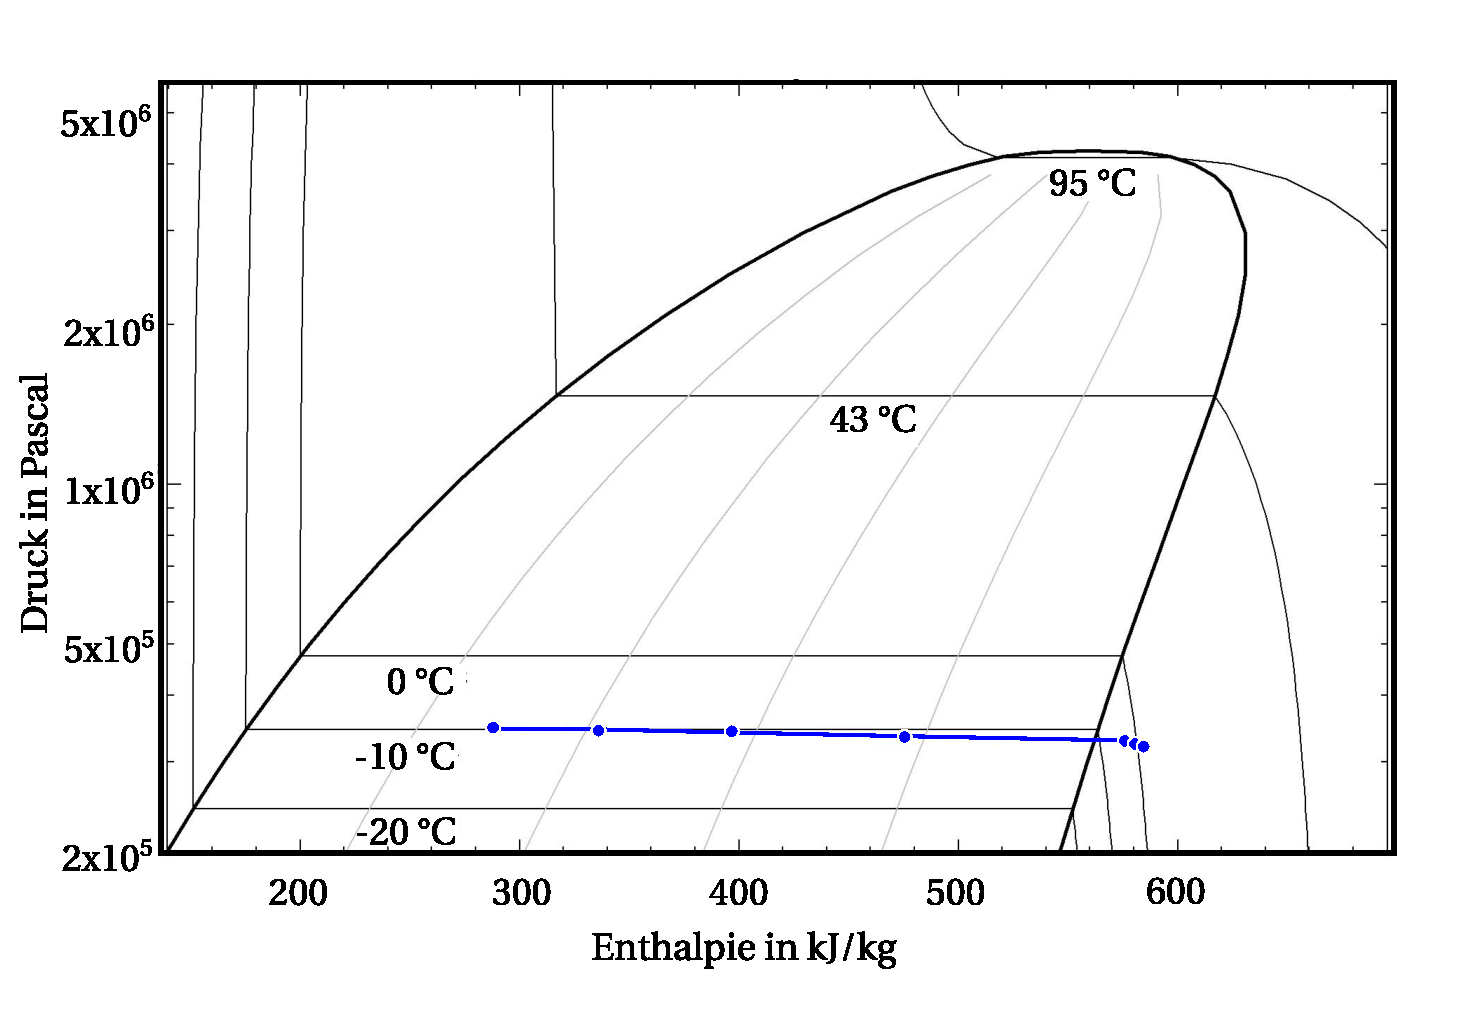
\includegraphics[scale=0.55]{Pictures/test61V1ogph.pdf}
%\caption{Simuliertes Druckprofil des Verdampfers für Verschaltung V1}
%\label{fig:SimDruckV1}
%\end{figure}

%\begin{figure}[h!]
%\centering
%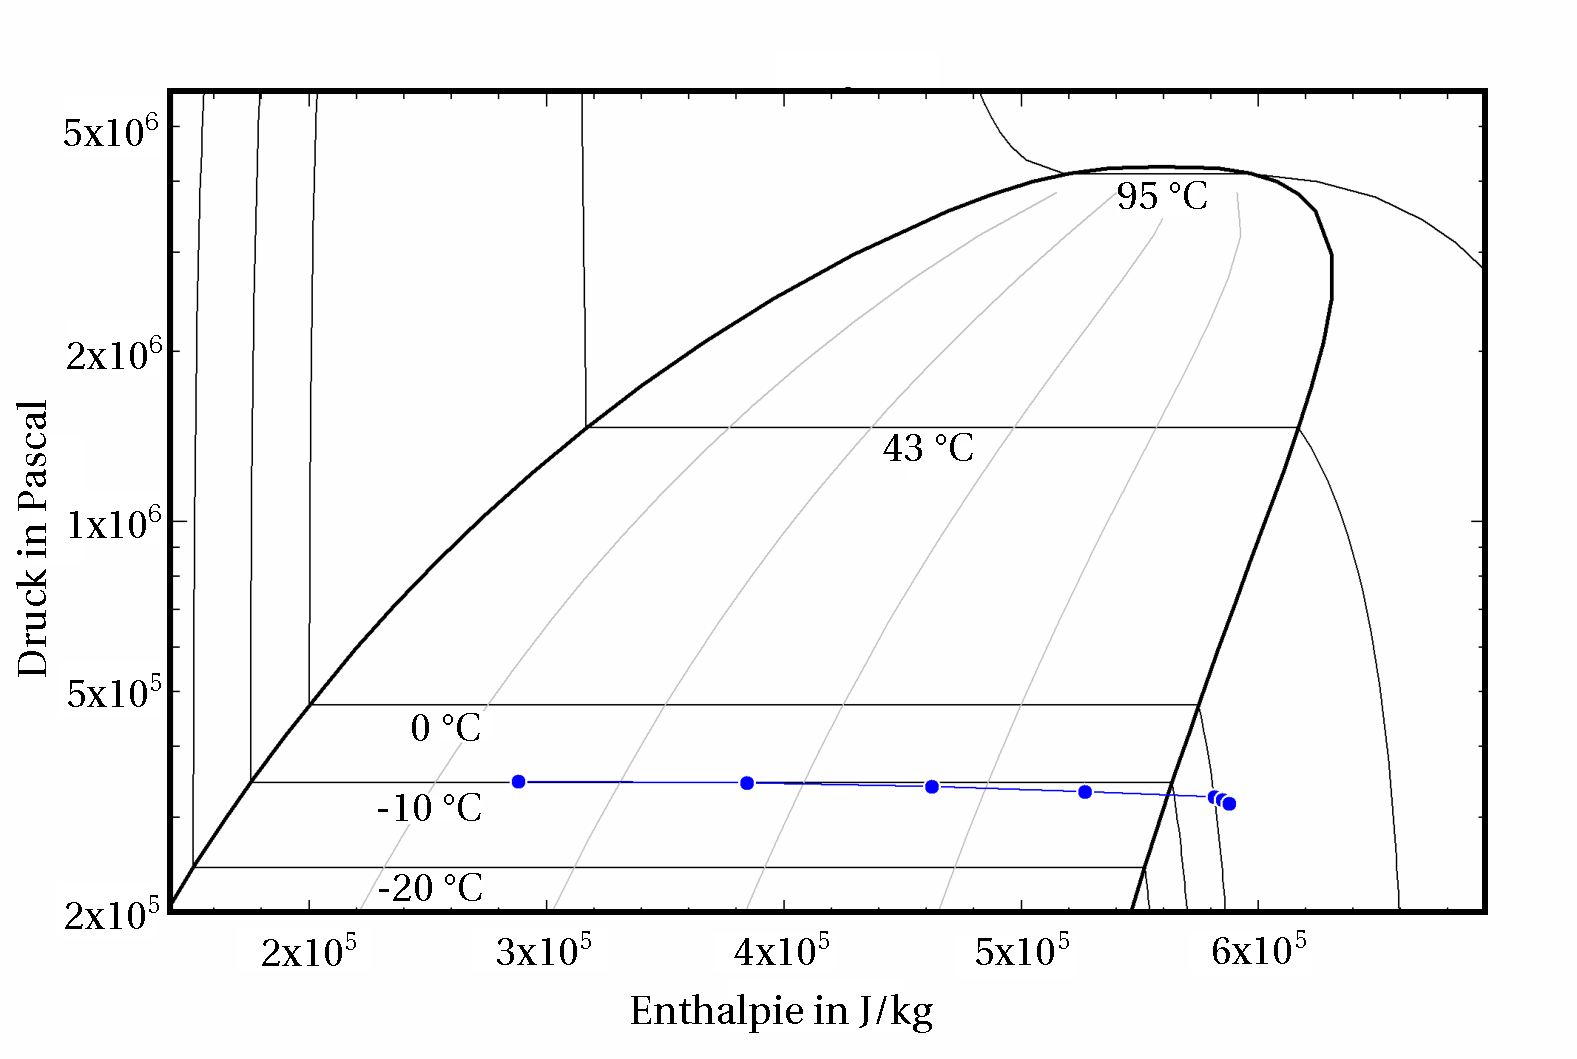
\includegraphics[scale=0.55]{Pictures/test61V2logph.pdf}
%\caption{Simuliertes Druckprofil des Verdampfers für Verschaltung V2}
%\label{fig:SimDruckV2}
%\end{figure}



